\documentclass[tikz,border=12pt]{standalone}
\usepackage{amsmath}
\usetikzlibrary{arrows.meta,angles,quotes}
\definecolor{avec}{RGB}{35,100,175}
\definecolor{bvec}{RGB}{195,70,45}
\definecolor{normal}{RGB}{30,130,95}
\begin{document}
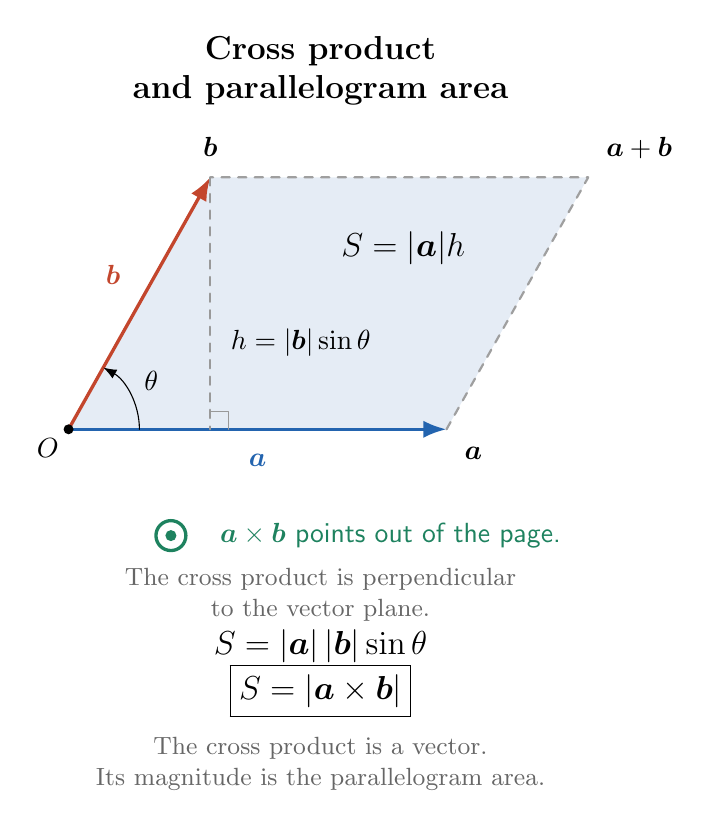
\begin{tikzpicture}[>=Latex,font=\sffamily,line cap=round,line join=round]
\coordinate (O) at (0,0);
\coordinate (A) at (4.8,0);
\coordinate (B) at (1.8,3.2);
\coordinate (C) at (6.6,3.2);
\coordinate (H) at (1.8,0);
\node[font=\large\bfseries] [align=center] at (3.2,4.55) {Cross product\\and parallelogram area};
\fill[avec!12] (O)--(A)--(C)--(B)--cycle;
\draw[gray!75,dashed,thick] (A)--(C)--(B);
\draw[avec,->,very thick] (O)--(A) node[midway,below=5pt] {$\boldsymbol a$};
\draw[bvec,->,very thick] (O)--(B) node[midway,above left=3pt] {$\boldsymbol b$};
\draw[gray!80,dashed,thick] (B)--(H);
\draw[gray!80] (1.8,.23)--(2.03,.23)--(2.03,0);
\node[anchor=west,fill=avec!12,inner sep=3pt] at (1.95,1.1) {$h=|\boldsymbol b|\sin\theta$};
\pic[draw,->,angle radius=9mm,angle eccentricity=1.35,"$\theta$"] {angle=A--O--B};
\node[align=center,font=\large] at (4.25,2.3) {$S=|\boldsymbol a|h$};
\fill (O) circle (1.8pt);
\node[below left] at (O) {$O$};
\node[above=4pt] at (B) {$\boldsymbol b$};
\node[above right=3pt] at (C) {$\boldsymbol a+\boldsymbol b$};
\node[below right=3pt] at (A) {$\boldsymbol a$};
% For the displayed orientation a to b is counterclockwise: a x b points out.

\draw[normal,very thick] (1.3,-1.35) circle (0.19);
\fill[normal] (1.3,-1.35) circle (2pt);
\node[normal,align=left,anchor=west] at (1.8,-1.35) {$\boldsymbol a\times\boldsymbol b$ points out of the page.};
\node[align=center,font=\small,text=gray!80!black] at (3.2,-2.1) {The cross product is perpendicular\\to the vector plane.};
\node[font=\large,align=center] at (3.2,-3.1) {$S=|\boldsymbol a|\,|\boldsymbol b|\sin\theta$\\$\boxed{S=|\boldsymbol a\times\boldsymbol b|}$};
\node[font=\small,align=center,text=gray!80!black] at (3.2,-4.25) {The cross product is a vector.\\Its magnitude is the parallelogram area.};
\end{tikzpicture}
\end{document}
